
\chapter{Probability}

Probability is the study of \textit{uncertainty}. This may seem like a
hopeless endeavor, sort of like knowing the unknowable, but it's not. The
study of probability gives us tools for taming the uncertain world we live
and program in, and for reasoning about it in a precise and helpful way.

We may not know exactly how long a particular visitor is willing to wait
for our webpage to load in their browser, but we can use probability to
estimate how much traffic we'll lose if this takes longer than a certain
average duration. We may not know which specific passwords a hacker will
try as he attempts to break our security protocol, but we can use
probability to estimate how feasible this approach will be for him. We may
not know exactly when a certain program will run out of RAM and have to
swap its data out to virtual memory, but we can predict how often this is
likely to occur --- and how painful it will be for us --- given a certain
system load and user behavior.

The trick is to use the tools we've already built --- sets, relations,
functions --- to characterize and structure our notions of the relative
likelihood of various outcomes. Once those underpinnings are secured, a
layer of deductive reasoning will help us make good use of that information
to begin to predict the future.

\section{Outcomes and events}

Since life is uncertain, we don't know for sure what is going to happen.
But let's start by assuming we know what things \textit{might} happen.
Something that might happen is called an \textbf{outcome}. You can think of
this as the result of an experiment if you want to, although normally we
won't be talking about outcomes that we have explicitly manipulated and
measured via scientific means. It's more like we're just curious how some
particular happening is going to turn out, and we've identified the
different ways it can turn out and called them outcomes.

\index{domain of discourse ($\Omega$)}
\index{sample space ($\Omega$)}
\index{outcomes}
Now we've been using the symbol $\Omega$ to refer to ``the domain of
discourse" or ``the universal set" or ``all the stuff we're talking about."
We're going to give it yet another name now: the \textbf{sample space}.
$\Omega$, the sample space, is simply \textit{the set of all possible
outcomes.} Any particular outcome --- call it $O$ --- is an element of this
set, just like in chapter 1 every conceivable element was a member of the
domain of discourse.

If a woman is about to have a baby, we might define $\Omega$ as \{~boy,
girl~\}. Any particular outcome $o$ is either boy or girl (not both),
but both outcomes are in the sample space, because both are possible. If we
roll a die, we'd define $\Omega$ as \{~1, 2, 3, 4, 5, 6~\}. If we're
interested in motor vehicle safety, we might define $\Omega$ for a
particular road trip as \{~safe, accident~\}. The outcomes don't have to be
equally likely, an important point we'll return to soon.

\index{events}
In probability, we define an \textbf{event} as \textit{a subset of the
sample space}. In other words, an event is a \textit{group} of related
outcomes (though an event might contain just one outcome, or even zero). I
always thought this was a funny definition for the word ``event": it's not
the first thing that word brings to mind. But it turns out to be a useful
concept, because sometimes we're not interested in any \textit{particular}
outcome necessarily, but rather in whether the outcome --- whatever it is
--- has a certain property. For instance, suppose at the start of some
game, my opponent and I each roll the die, agreeing that the highest roller
gets to go first. Suppose he rolls a 2. Now it's my turn. The $\Omega$ for
my die roll is of course \{~1, 2, 3, 4, 5, 6~\}. But in this case, it
doesn't necessarily matter what my specific outcome is; only whether I beat
a 2. So I could define the \textit{event} $M$ (for ``me first") to be the
set \{~3, 4, 5, 6~\}. I could define the event $H$ (``him first") to be the
set \{~1~\} (notice $H$ is still a set, even though it has only one
element.) Then I could define the event $T$ (``tie") as the set \{~2~\}.
I've now effectively collapsed a larger set of outcomes into only the
groups of outcomes I'm interested in. Now I'm all ready to reason about the
likelihood that each of these events actually occurs.

By the way, ``the set of all outcomes" is simply $\Omega$, since an outcome
is an element of $\Omega$. But an event is a \textit{subset} of $\Omega$,
not a single element. What, then, is ``the set of all events?" If you think
it through, you'll realize that it's $\mathbb{P}(\Omega)$ (the
\textit{power set} of the sample space). Put another way, when defining an
event, I can choose any subset of the possible outcomes, and so I can
choose any set from $\mathbb{P}(\Omega)$.

\section{Probability measures}

\index{probability measures}
\index{functions}
\index{interval}
\index{closed interval}
\index{events}

Okay, we've defined sample spaces and events, but when do quantitative
notions like ``the odds of" and ``percent chance" come into play? They
enter the scene when we define a \textbf{probability measure}. A
probability measure is simply \textit{a function from the domain of events
to the codomain of real numbers.} We'll normally use the letters ``Pr" for
our probability measure. In symbols, $\text{Pr}:\mathbb{P}(\Omega) \to
\mathbb{R}$ (since the set of all events is the power set of the sample
space, as per above). There's actually another constraint, though, which is
that Pr's values must be in the range 0 to 1, inclusive. So it's more
correct to write: $\text{Pr}:\mathbb{P}(\Omega)\to [0,1]$. (You may recall
from a previous math course that `[' and `]' are used to describe a closed
interval in which the endpoints are included in the interval.)

The ``meaning" of the probability measure is intuitive enough: it indicates
how likely we think each event is to occur. In the baby example, if we say
Pr(\{boy\}) = .5, it means there's a .5 probability (a.k.a., a 50\% chance)
that a male child will be born. In the game example, if we say Pr($M$) =
.667, if means there's a two-thirds chance of me winning the right to go
first. In all cases, a probability of 0 means ``impossible to occur" and a
probability of 1 means ``absolutely certain to occur." In colloquial
English, we most often use percentages to talk about these things: we'll
say ``there's a 60\% chance Obama will win the election" rather than
``there's a .6 probability of Obama winning." The math's a bit clumsier
if we deal with percentages, though, so from now on we'll get in the
habit of using probabilities rather than `percent chances,' and we'll use
values in the 0 to 1 range rather than 0 to 100.

\index{outcomes}
I find the easiest way to think about probability measures is to start with
the probabilities of the \textit{outcomes}, not events. Each outcome has a
specific probability of occuring. The probabilities of events logically
flow from that just by using addition, as we'll see in a moment. 

\index{American Idol}
For example, let's imagine that Fox Broadcasting is producing a worldwide
television event called \textit{All-time Idol}, in which the yearly winners
of \textit{American Idol} throughout its history all compete against each
other to be crowned the ``All-time American Idol champion." The four
contestants chosen for this competition, along with their musical genres,
and age when originally appearing on the show, are as follows:

\begin{minipage}{\textwidth}
\begin{center}
Kelly Clarkson (20): pop, rock, R\&B \\
Fantasia Barrino (20): pop, R\&B \\
Carrie Underwood (22): country \\
David Cook (26): rock
\end{center}
\end{minipage}

Entertainment shows, gossip columns, and \textit{People} magazine are all
abuzz in the weeks preceding the competition, to the point where a shrewd
analyst can estimate the probabilities of each contestant winning. Our
current best estimates are: Kelly .2, Fantasia .2, Carrie .1, and David .5.

Computing the probability for a specific event is just a matter of adding
up the probabilities of its outcomes. Define $F$ as the event that a woman
wins the competition. Clearly Pr($F$) = .5, since Pr(\{Kelly\}) = .2,
Pr(\{Fantasia\}) = .2, and Pr(\{Carrie\}) = .1. If $P$ is the event that a
rock singer wins, Pr($P$) = .7, since this is the sum of Kelly's and
David's probabilities.

Now it turns out that not just \textit{any} function will do as a
probability measure, even if the domain (events) and codomain (real numbers
in the range[0,1]) are correct. In order for a function to be a ``valid"
probability measure, it must satisfy several other rules:
\index{probability measures}
\begin{enumerate}
\item \label{somethinghappens} $\text{Pr}(\Omega) = 1$
\item \label{nonegs} $\text{Pr}(A) \geq 0$ for all $A \subseteq \Omega$
\item \label{probunion} $\text{Pr}(A \cup B) = \text{Pr}(A) + \text{Pr}(B) -
    \text{Pr}(A \cap B)$
\end{enumerate}

Rule~\ref{somethinghappens} basically means ``\textit{something} has to
happen." If we create an event that includes every possible outcome, then
there's a probability of 1 (100\% chance) the event will occur, because
after all \textit{some} outcome has got to occur. (And of course
Pr($\Omega$) can't be \textit{greater} than 1, either, because it doesn't
make sense to have any probability over 1.) Rule~\ref{nonegs} says there's
no negative probabilities: you can't define any event, no matter how
remote, that has a less than zero chance of happening.

\index{additivity property}
\index{Venn diagrams}
Rule~\ref{probunion} is called the ``additivity property," and is a bit
more difficult to get your head around. A diagram works wonders. Consider
Figure~\ref{venn}, called a ``Venn diagram," which visually depicts sets
and their contents. Here we have defined three events: $F$ (as above) is
the event that the winner is a woman; $R$ is the event that the winner is a
rock musician (perhaps in addition to other musical genres); and $U$ is the
event that the winner is underage (\textit{i.e.}, becomes a multimillionare
before they can legally drink). Each of these events is depicted as a
closed curve which encloses the outcomes that belong to it. There is
obviously a great deal of overlap.

\begin{figure}[ht]
\centering
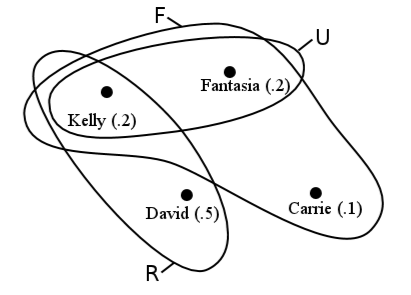
\includegraphics[width=0.7\textwidth]{idol.png}
\caption{Various events, and their overlap.}
\label{venn}
\end{figure}

\index{inclusive or}
\index{exclusive or}
Now back to rule~\ref{probunion}. Suppose I ask ``what's the probability
that the All-time Idol winner is underage or a rock star?" Right
away we face an irritating ambiguity in the English language: does ``or"
mean ``\textit{either} underage \textit{or} a rock star, but not both?" Or
does it mean ``underage \textit{and/or} rock star?" The former
interpretation is called an \textbf{exclusive or} and the latter an
\textbf{inclusive or}. In computer science, we will almost always be
assuming an \textit{inclusive} or, unless explicitly noted otherwise.

Very well then. What we're really asking here is ``what's Pr($U \cup R$)?"
We want the union of the two events, since we're asking for the probability
that \textit{either} (or both) of them occurs. You might first think that
we'd add the two probabilities for the two events and be done with it, but
a glance at the diagram tells you this means trouble. Pr($U$) is .4, and
Pr($R$) is .7. Even if we weren't very smart, we'd know something was wrong
as soon as we added $.4 + .7 = 1.1$ to get a probability of over 1 and
violate rule~\ref{somethinghappens}. But we are smart, and looking at the
diagram it's easy to see what happened: \textit{we double-counted Kelly's
probability.} Kelly was a member of both groups, so her .2 got counted in
there twice. Now you can see the rationale for rule~\ref{probunion}. To get
Pr($U \cup R$) we add Pr($U$) and Pr($R$), but then we have to subtract
back out the part we double-counted. And what did we double-count?
Precisely the intersection $U \cap R$.

As a second example, suppose we want the probability of an underage or
female winner? Pr($U$) = .4, and Pr($F$) = .5, so the first step is to just
add these. Then we subtract out the intersection, which we double counted.
In this case, the intersection $U \cap F$ is just $U$ (check the diagram),
and so subtract out the whole .4. The answer is .5, as it should be.

By the way, you'll notice that if the two sets in question are mutually
exclusive, then there is no intersection to subtract out. That's a special
case of rule~\ref{probunion}. For example, suppose I defined the event $C$
as a country singer winning the competition. In this case, $C$ contains
only one outcome: Carrie. Therefore $U$ and $C$ are mutually exclusive. So
if I asked ``what's the probability of an underage or country winner?" we'd
compute Pr($U \cup C$) as 

\begin{align*}
\text{Pr}(U \cup C) &= \text{Pr}(U) + \text{Pr}(C) - \text{Pr}(U \cap C) \\
&= .4 + .1 - 0 \\
&= .5.
\end{align*}

We didn't double-count anything, so there was no correction to make.

Here are a few more pretty obvious rules for probability measures, which
follow logically from the first \ref{probunion}:

\index{probability measures}
\begin{enumerate}[resume]
\item Pr($\varnothing$) = 0 
\index{complement, total (of sets)}
\item Pr($\overline{A}$) = $1-$Pr($A$) \quad (recall the ``total complement"
operator from p.~\pageref{complement}.)
\item Pr($A$) $\leq$ Pr($B$) if $A \subseteq B$
\end{enumerate}

Finally, let me draw attention to a common special case of the above rules,
which is the situation in which all outcomes are equally likely. This
usually happens when we roll dice, flip coins, deal cards, \textit{etc.}
since the probability of rolling a 3 is (normally) the same as rolling a 6,
and the probability of being dealt the 10$\spadesuit$ is the same as the
Q$\diamondsuit$. It may also happen when we generate encryption keys,
choose between alternate network routing paths, or determine the initial
positions of baddies in a first-person shooter level.

In this case, if there are $N$ possible outcomes (note $N=|\Omega|$) then
the probability of any event A is:

\begin{center}
Pr($A$) = $\dfrac{|A|}{N}$.
\end{center}

\index{cardinality (of sets)}
It's the size (cardinality) of the event set that matters, and the ratio of
this number to the total number of events is the probability. For example,
if we deal a card from a fair deck, the probability of drawing a face card
is

\begin{align*}
\text{Pr}(F) &= \frac{|F|}{N} \\[.1in]
&= \frac{|\{K\spadesuit,K\heartsuit,K\diamondsuit,\cdots,J\clubsuit\}|}{52} \\[.1in]
&= \frac{12}{52} = .231.
\end{align*}

Please realize that this shortcut \textit{only} applies when the
probability of each outcome is the same. We certainly couldn't say, for
example, that the probability of a user's password starting with the letter
\texttt{q} is just $\frac{1}{26}$, because passwords surely don't contain
all letters with equal frequency. (At least, I'd be very surprised if that
were the case.) The only way to solve a problem like this is to know how
often each letter of the alphabet occurs.

\section{Philosophical interlude}

Which brings me to an important question. How do we get these probability
numbers, anyway? Everything so far has assumed that the numbers have been
dropped into our lap.

\index{frequentist}
\index{Bayesian}
The answer depends somewhat on your interpretation of what probability
\textit{means}. If we say ``the probability of getting heads on a coin flip
is .5," what are we really saying? There have traditionally been two
opposing answers to this question, called the \textbf{frequentist} view and
the \textbf{Bayesian} view. It's interesting to compare their claims.

The frequentist view is that we derive probabilities by simply running many
trials, and counting the results. The proportions of various outcomes yield
a good idea of their probabilities, particularly if the sample size is
large. Consider flipping a coin. If we flip a coin ten times and count
three heads, we might not have a great idea of how often heads will occur
in the long run. But if we flip it a million times and get 500,372 heads,
we can confidently say that the probability of getting a head on a single
flip is approximately .500.

\index{Venn, John}
\index{Fisher, Ronald}
This much isn't controversial: it's more like common sense. But the
frequentist philosophy states that this is really the \textit{only} way
that probability can be defined. It's what probability \textit{is}: the
frequency with which we can expect certain outcomes to occur, based on our
observations of their past behavior. Probabilities only make sense for
things that are repeatable, and reflect a known, reliable trend in how
often they produce certain results. Historical proponents of this
philosophy include John Venn, the inventor of the aforementioned Venn
diagram, and Ronald Fisher, one of the greatest biologists and
statisticians of all time.

If frequentism is thus on a quest for experimental objectivity, Bayesianism
might be called ``subjective." This isn't to say it's arbitrary or sloppy.
It simply has a different notion of what probability ultimately means.
Bayesians interpret probability as a quantitative personal assessment of
the likelihood of something happening. They point out that for many (most)
events of interest, trials are neither possible nor sensible. Suppose I'm
considering asking a girl out to the prom, and I'm trying to estimate how
likely it is she'll go with me. It's not like I'm going to ask her a
hundred times and count how many times she says yes, then divide by 100 to
get a probability. There is in fact no way to perform a trial or use past
data to guide me, and at any rate she's only going to say yes or no once.
So based on my background knowledge and my assumptions about her, myself,
and the world, I form an opinion which could be quantified as a ``percent
chance."

\index{Laplace, Pierre-Simon}
\index{Newton, Isaac}
\index{Bayes, Thomas}
Once I've formed this opinion (which of course involves guesswork and
subjectivity) I can then reason about it mathematically, using all the
tools we've been developing. Of special interest to Bayesians is the notion
of \textit{updating} probabilities when new information comes to light, a
topic we'll return to in a moment. For the Bayesian, the probability of
some hypothesis being true is between 0 and 1, and when an agent (a human,
or a bot) makes decisions, he/she/it does so on the most up-to-date
information he/she/it has, always revising beliefs in various hypotheses
when confirming or refuting evidence is encountered. Famous Bayesians
include Pierre-Simon Laplace, sometimes called ``the French Isaac Newton"
for his scientific brilliance, and $18{^{\text{th}}}$ century theologian
Thomas Bayes, for whom the theory is named.

I won't try to conceal that my own thinking on this topic is pretty
Bayesian. But I find this whole topic fascinating because it shows how
brilliant people, who unanimously agree on the rules and equations, can
have such radically different interpretations of what it all means.


\section{Conditional probability}

\index{conditional probability}
I mentioned that Bayesians are especially concerned with the idea of
revising estimates about probability based on new information that may come
to light. This notion can be crystallized in the idea of
\textbf{conditional probability}. When we talk about the conditional
probability of an event $A$, we mean ``what's the probability that $A$
occurs, \textit{given} that I know some other event $K$ has also occurred?"
Think of $K$ as ``background knowledge": it's additional information which,
when known, may influence how likely we think $A$ is to have occurred. It
can be mathematically computed as follows:

\[
\text{Pr}(A|K) = \dfrac{\text{Pr}(A \cap K)}{\text{Pr}(K)}
\]

\index{prior probability}
\index{background knowledge}
\index{\textit{a priori}}
We pronounce Pr($A|K$) as ``the probability of $A$ given $K$." It is the
conditional probability of $A$, or ``the probability of $A$ conditioned on
$K$." We'll sometimes call plain old Pr($A$) the \textbf{\textit{a priori}
probability}, or the \textbf{prior} probability if we don't want to sound
Latin. The prior is simply the original unadjusted probability, if we
aren't privy to the background information $K$.

\index{American Idol}
Let's go back to \textit{American Idol}. We know that the probability of an
underage winner is only .4, because $U$ = \{~Kelly, Fantasia~\}, and we
estimate that each of them has a .2 probability of winning. So it seems
more likely than not that our winner will be over 21. But wait: suppose we
had some additional information. Just before the outcome is announced, news
is leaked through a Rupert Murdoch news source that the winner is a
\textit{woman}! If we believe this reporter, does that change our
expectation about how old the winner is likely to be?

Indeed it does. Knowing that the winner is female eliminates Dave from
consideration. Looking back at Figure~\ref{venn}, we can see that once we
know Dave is out of the running, the remaining pool consists of just $F$,
which includes Kelly, Fantasia, and Carrie. The question is, how do we
update our probability from .4 to reflect the fact that only these three
ladies are 

In this case $F$ is the background knowledge: we know that the event $F$
has occurred. And we want to know how likely $U$ is to also have occurred.
This is found easily:

\begin{align*}
\text{Pr}(U|F) &= \dfrac{\text{Pr}(U \cap F)}{\text{Pr}(F)} \\
&= \dfrac{\text{Pr}(\{\text{Kelly,Fantasia}\})}{\text{Pr}(\{\text{Kelly,Fantasia,Carrie}\})}
\\
&= \dfrac{.4}{.5} = .8.
\end{align*}

Our estimated chance of an underage winner doubled once we found out she
was female (even though we don't yet know \textit{which} female).

If you stare at the equation and diagram, you'll see the rationale for this
formula. Kelly and Fantasia originally had only .4 of the entire
probability between them. But once David was axed, the question became:
``what percentage of the \textit{remaining} probability do Kelly and
Fantasia have?" The answer was no longer .4 out of 1, but .4 out of .5,
since only .5 of the whole was left post-David. This is why we divided by
Pr($F$): that's what we know remains given our background fact.

Now in this case, the conditional probability was higher than the original
probability. Could it ever be lower? Easily. Consider the probability of a
rock-star winner, Pr($R$). \textit{A priori}, it's .7. But again, let's say
we had information leaked to us that the winner, whoever she may be, is
female. We can now update our estimate:

\begin{align*}
\text{Pr}(R|F) &= \dfrac{\text{Pr}(R \cap F)}{\text{Pr}(F)} \\
&= \dfrac{\text{Pr}(\{\text{Kelly}\})}{\text{Pr}(\{\text{Kelly,Fantasia,Carrie}\})}
\\
&= \dfrac{.2}{.5} = .4.
\end{align*}

You see, once we find out that David is no longer a possibility, our only
remaining hope for a rock star is Kelly. And she has only 40\% of the
probability that's left over. Note that this is a higher chance for
her personally --- she's got to be excited by the press leak --- but it's
lower for \textit{rock stars}, of which she is only one (and evidently, not
the predicted strongest).

\index{background knowledge}
Background knowledge can even peg our probability estimate to an extreme:
all the way to 0, or to 1. What's Pr($U|C$), the probability of an underage
winner, given that he/she is a country singer? The intersection of $U$ and
$C$ is zero, so this makes Pr($U|C$) = 0. In words: a country winner
eliminates any possibility of an underage winner. And what's Pr($F|U$), the
probability that a woman wins, given that we know the winner to be
underage? Well, $F \cap U$ and $U$ are the same (check me), so
$\frac{\text{Pr}(F \cap U)}{\text{Pr}(U)} = \frac{.4}{.4} = 1$. Therefore,
an underage winner guarantees a female winner.

The way I think about conditional probability is this: look at the diagram,
consider the events known to have occurred, and then \textit{mentally block
out everything except that.} Once we know the background fact(s), we're
essentially dealing with a restricted world. Take the example of the known
female winner. Once we know that event $F$ in fact occurred, we can
visually filter out David, and look at the $F$ blob as though that were our
entire world. In this restricted female-only view, the underage elements
comprise a greater percentage of the total than they did before. And half
of the rock-star elements have now been obscured, leaving only Kelly as the
one-of-the-remaining-three.

\index{psychology}
Many psychologists, by the way, claim that we're constantly doing this sort
of thing in our minds: gathering facts, then revising our beliefs about the
world in light of those facts. We start by believing that Pr($X$) is
approximately some value. Then we learn $K_1$ has occurred, and we update
this to Pr($X|K_1$). Then we learn that $K_2$ has also occurred, and so now
we have Pr($X|K_1 \cap K_2$). (Can you see why it's the intersection?) The
more we learn, the more we revise our estimate up or down, presumably
getting more accurate as we go. Another way of looking at it is that every
time we learn something new is true, we also learn that its opposite is
\textit{not} true, and therefore we can eliminate some parts of the
theoretically-possible universe that we have now ruled out. The denominator
gets smaller and smaller as we eliminate possibilities.

\index{commutative}
Keep in mind, by the way, that unlike union and intersection, conditional
probability is not commutative. In other words, Pr($X|Y$) $\neq$ Pr($Y|X$)
in general. To take just one example, look again at the $F$ and $U$ sets
from \textit{All-time Idol}. Pr($F|U$), as we already computed, is equal to
1 since if $U$ has occurred, we automatically know that $F$ has also
occurred (there aren't any underage contestants \textit{except} females).
But the reverse is certainly not true: just because we have a female
winner doesn't mean we have an underage winner, since the winner might be
Carrie. Working it out, Pr($U|F$) = $\frac{\text{Pr}(U \cap
F)}{\text{Pr}(F)} = \frac{.4}{.5} = .8$. Higher than Pr($U$), but not 1.

\section{Total probability}
\label{totalprob}

\index{Law of Total Probability}
There's a very useful fact that goes by the grandiose name ``The Law of
Total Probability." It goes like this. If there's an event whose
probability we'd like to know, we can split it up into pieces and add up
their probabilities, as long as we do it in the right way.

\index{partitions}
``The right way" bit is the key, of course. And it has to do with
partitions. Recall from section~\ref{partitions} that a partition of a set
is a mutually exclusive and collectively exhaustive group of subsets. One
example is that \textit{every} set and its complement together form a
partition of $\Omega$. By the same token, for any sets $A$ and $B$, these
two sets together form a partition of $A$:

\begin{align*}
A \cap B \\
A \cap \overline{B}
\end{align*}

\index{WWE wrestling}
\index{southern states}
This is worth taking a moment to understand completely. Suppose $A$ is the
set of all WWE professional wrestling fans, and $B$ is the set of all
people born in southern states. The first set listed above, $A \cap B$
contains professional wrestling fans born in southern states, and the
second set, $A \cap \overline{B}$, the wrestling fans not born in southern
states.  Clearly, every wrestling fan is in one of these two sets, and no
fan is in both. So it's a partition of $A$. This works for \textit{any} two
sets $A$ and $B$: $A \cap B$ and $A \cap \overline{B}$ are a partition of
$A$. We're just dividing up the A's into the A's that are also B's, and the
A's that are not B's. Every A is in one (and just one) of those groups.

This idea can be extended to more than two sets. Let $C_1$ be the set of
all people born in southern states, $C_2$ the set of people born in western
states, and $C_3$ those not born in either region. (The set $C_3$ includes
lots of things: people born in Ohio, people born in Taiwan, and ham
sandwiches, among others.) The following three sets, then, together form
another partition of $A$: $A \cap C_1$, $A \cap C_2$, and $A \cap C_3$.
This is because every professional wrestling fan is either born in the
south, or born in the west, or neither one. 

Okay, now back to probability. In the two-set case, no matter what the
event $A$ is, we can divide up its probability like this:

\begin{align*}
\text{Pr}(A) &= \text{Pr}(A \cap B) + \text{Pr}(A \cap \overline{B}) \\
&= \text{Pr}(A|B) \text{Pr}(B) + \text{Pr}(A|\overline{B}) \text{Pr}(\overline{B})
\end{align*}

\index{conditional probability}
where $B$ is any other event. The last step makes use of the conditional
probability definition from above. We're dividing up A into the B's and the
non-B's, in a strategy to determine A's probability. In the general case,
if $N$ sets named $C_k$ (where $k$ is a number from 1 to $N$) make up a
partition of $\Omega$, then:

\begin{align*}
\text{Pr}(A) &= \text{Pr}(A \cap C_1) +
\text{Pr}(A \cap C_2) + 
\cdots +
\text{Pr}(A \cap C_N) \\
&= \text{Pr}(A|C_1) \text{Pr}(C_1) +
\text{Pr}(A|C_2) \text{Pr}(C_2) +
\cdots +
\text{Pr}(A|C_N) \text{Pr}(C_N) \\
&= \sum_{k=1}^N{\text{Pr}(A|C_k) \text{Pr}(C_k)}
\end{align*}

\index{summation operator ($\Sigma$)}
is the formula.\footnote{If you're not familiar with the notation in that
last line, realize that $\Sigma$ (a capital Greek ``sigma") just represents
a sort of loop with a counter. The ``$k=1$" under the sign means that the
counter is $k$ and starts at 1; the ``$N$" above the sign means the counter
goes up to $N$, which is its last value. And what does the loop do? It adds
up a cumulative sum. The thing being added to the total each time through
the loop is the expression to the right of the sign. The last line with the
$\Sigma$ is just a more compact way of expressing the preceding line.}

\index{movie theatre}
\index{Avengers, The}
\index{Black Swan}
\index{Dr. Seuss}
Let's take an example of this approach. Suppose that as part of a promotion
for Muvico Cinemas movie theatre, we're planning to give a door prize to
the $1000^{\text{th}}$ customer this Saturday afternoon. We want to know,
though, the probability that this person will be a minor. Figuring out how
many patrons overall will be under 18 might be difficult. But suppose we're
showing these three films on Saturday: The Avengers, Black Swan, and Dr.
Seuss's The Lorax. We can estimate the fraction of each movie's viewers
that will be minors: .6, .01, and .95, respectively. We can also predict
how many tickets will be sold for each film: 2,000 for the Avengers, 500
for Black Swan, and 1,000 for Lorax.

Applying frequentist principles, we can compute the probability that a
particular visitor will be seeing each of the movies:

\begin{center}
Pr(Avengers) = $\frac{2000}{2000+500+1000} = .571$ \\[.1in]
Pr(BlackSwan) = $\frac{500}{2000+500+1000} = .143$\\[.1in]
Pr(Lorax) = $\frac{1500}{2000+500+1000} = .286$
\end{center}

To be clear: this is saying that if we select a visitor at random on
Saturday, the probability that they will be seeing The Avengers is .571.

\index{conditional probability}
But (and this is the trick) we can also compute the \textit{conditional}
probability that an attendee of each of these films will be a minor:

\begin{align*}
\text{Pr(minor}|\text{Avengers)} &= .6 \\
\text{Pr(minor}|\text{BlackSwan)} &= .01 \\
\text{Pr(minor}|\text{Lorax)} &= .95
\end{align*}

In words: ``If we know that a visitor is coming to see The Avengers,
there's a .6 probability that they'll be a minor." We're using the
background knowledge to determine the conditional probability. It might be
hard to figure out the probability of minors in general, but easier to
figure out the probability of minors watching a specific movie.

Now, it's just a matter of stitching together the parts:

\begin{align*}
\text{Pr(minor)} = &\ \text{Pr(minor}|\text{Avengers) Pr(Avengers)} +  \\
&\ \text{Pr(minor}|\text{BlackSwan) Pr(BlackSwan)} +  \\
&\ \text{Pr(minor}|\text{Lorax) Pr(Lorax)}\\
= &\ .6 \cdot .571 + .01 \cdot .143 + .95 \cdot .286 \\
= &\ .343 + .00143 + .272 \approx .616
\end{align*}

In words, there are three different ways for a visitor to be a minor: they
could be an Avengers fan and a minor (pretty likely, since there's lots of
Avengers fans), or a Black Swan fan and a minor (not likely), or a Lorax
fan and a minor (fairly likely, since although there's not a ton of Lorax
fans overall, most of them are minors). Adding up these probabilities is
legit only \textit{because} the three movies form a partition of the
visitors (\textit{i.e.}, every visitor is there to see one and only one
movie).

The Law of Total Probability comes in handy in scenarios where there's more
than one ``way" for an event to occur. It lets you break that event apart
into the different ways, then apply your knowledge of the likelihood of
each of those ways in order to compute the grand, overall probability of
the event.


\section{Bayes' Theorem}
\index{Bayes' Theorem}

Another trick that helps compute probabilities in practice is
\textbf{Bayes' Theorem.} We've defined Pr($A|K$) as $\frac{\text{Pr}(A \cap
K)}{\text{Pr}(K)}$, and by swapping the letters we get Pr($K|A$) =
$\frac{\text{Pr}(K \cap A)}{\text{Pr}(A)}$. Combining these with a little
bit of algebra yields:

\begin{align*}
\text{Pr}(A|K) = \dfrac{\text{Pr}(K|A) \ \text{Pr}(A)}{\text{Pr}(K)}
\end{align*}

Now this is a very, very powerful equation that has a multitude of uses
throughout computer science and statistics. What makes it powerful is that
it allows us to express Pr($A|K$), a quantity often very difficult to
estimate, in terms of Pr($K|A$), which is often much easier.

\index{medical test}
A simple and commonly cited example is that of interpreting medical exam
results for the presence of a disease. If your doctor recommends that you
undergo a blood test to see if you have some rare condition, you might test
positive or negative. But suppose you do indeed test positive. What's the
probability that you actually have the disease? That, of course, is the key
point.

In symbols, we're looking for Pr($D|T$), where $D$ is the event that you
actually have the disease in question, and $T$ is the event that you test
positive for it. But this is hard to approximate with available data. For
one thing, most people who undergo this test \textit{don't} test positive,
so we don't have a ton of examples of event $T$ occurring whereby we could
count the times $D$ also occurred. But worse, it's hard to tell whether a
patient \textit{has} the disease, at least before advanced symptoms develop
--- that, after all, is the purpose of our test!

Bayes' Theorem, however, lets us rewrite this as:

\begin{align*}
\text{Pr}(D|T) = \dfrac{\text{Pr}(T|D) \ \text{Pr}(D)}{\text{Pr}(T)}.
\end{align*}

Now we have Pr($D|T$), the hard quantity to compute, in terms of three
things we \textit{can} get data for. To estimate Pr($T|D$), the probability
of a person who has the disease testing positive, we can administer the
test to unfortunate patients with advanced symptoms and count how many of
them test positive. To estimate Pr($D$), the prior probability of having
the disease, we can divide the number of known cases by the population as a
whole to find how prevalent it is. And getting Pr($T$), the probability of
testing positive, is easy since we know the results of the tests we've
administered.

In numbers, suppose our test is 99\% accurate --- \textit{i.e.}, if someone
actually has the disease, there's a .99 probability they'll test positive
for it, and if they don't have it, there's a .99 probability they'll test
negative. Let's also assume that this is a very rare disease: only one in a
thousand people contracts it.

When we interpret those numbers in light of the formula we're seeking to
populate, we realize that Pr($T|D$) = .99, and Pr($D$) = $\frac{1}{1000}$.
The other quantity we need is Pr($T$), and we're all set. But how do we
figure out Pr($T$), the probability of testing positive?

\index{Law of Total Probability}
Answer: use the Law of Total Probability. There are two different ``ways" to
test positive: (1) to actually have the disease, and (correctly) test
positive for it, or (2) to \textit{not} have the disease, but incorrectly
test positive for it anyway because the test was wrong. Let's compute this:

\begin{align}
\text{Pr}(T) &=
    \text{Pr}(T|D) \ \text{Pr}(D) + 
    \text{Pr}(T|\overline{D}) \ \text{Pr}({\overline{D}}) \notag \\
&= .99 \cdot \frac{1}{1000} + .01 \cdot \frac{999}{1000} \notag \\
&= .00099 + .00999 = .01098  \label{totalprobeq}
\end{align}

\index{mutually exclusive}
See how that works? If I \textit{do} have the disease (and there's a 1 in
1,000 chance of that), there's a .99 probability of me testing positive. On
the other hand, if I \textit{don't} have the disease (a 999 in 1,000 chance
of that), there's a .01 probability of me testing positive anyway. The sum
of those two mutually exclusive probabilities is .01098.

Now we can use our Bayes' Theorem formula to deduce:

\begin{align*}
\text{Pr}(D|T) &= \dfrac{\text{Pr}(T|D) \ \text{Pr}(D)}{\text{Pr}(T)} \\
&= \dfrac{.99 \cdot \frac{1}{1000}}{.01098} \approx .0902
\end{align*}

Wow. We tested positive on a 99\% accurate medical exam, yet we only have
about a 9\% chance of actually having the disease! Great news for the
patient, but a head-scratcher for the math student. How can we understand
this? Well, the key is to look back at that Total Probability calculation
in equation~\ref{totalprobeq}. Remember that there were two ways to test
positive: one where you had the disease, and one where you didn't. Look at
the contribution to the whole that each of those two probabilities
produced.  The first was .00099, and the second was .00999, over ten times
higher. Why? Simply because the disease is so rare. Think about it: the
test fails once every hundred times, but a random person only has the
disease once every \textit{thousand} times. If you test positive, it's far
more likely that the test screwed up than that you actually have the
disease, which is rarer than blue moons.

Anyway, all the stuff about diseases and tests is a side note. The main
point is that Bayes' Theorem allows us to recast a search for Pr($X|Y$)
into a search for Pr($Y|X$), which is often far easier to find numbers for.

\index{text mining}
\index{Federalist Papers}
\index{Hamilton, Alexander}
\index{Madison, James}
\index{Jay, John}
One of many computer science applications of Bayes' Theorem is in text
mining. In this field, we computationally analyze the words in documents in
order to automatically classify them or form summaries or conclusions about
their contents. One goal might be to identify the true author of a
document, given samples of the writing of various suspected authors.
Consider the \textit{Federalist Papers}, the group of highly influential
$18^{th}$ century essays that argued for ratifying the Constitution. These
essays were jointly authored by Alexander Hamilton, James Madison, and John
Jay, but it was uncertain for many years which of these authors wrote which
specific essays.

Suppose we're interested in determining which of these three Founding
Fathers actually wrote essay \#84 in the collection. To do this, the
logical approach is to find Pr(Hamilton$|$essay84), Pr(Madison$|$essay84),
and Pr(Jay$|$essay84), and then choose the author with the highest
probability.  But how can we possibly find out Pr(Hamilton$|$essay84)?
``Given that essay \#84 has these words in this order, what's the
probability that Hamilton wrote it?" Impossible to know.

But with Bayes' Theorem, we can restructure this in terms of
Pr(essay84$|$Hamilton) instead. That's a horse of a different color. We
have lots of known samples of Hamilton's writing (and Madison's, and
Jay's), so we can ask, ``given that Hamilton wrote an essay, what's the
probability that he would have chosen the words that appear in essay \#84?"
Perhaps essay \#84 has a turn of phrase that is very characteristic of
Hamilton, and contains certain vocabulary words that Madison never used
elsewhere, and has fewer sentences per paragraph than is typical of Jay's
writing. If we can identify the relevant features of the essay and compare
them to the writing styles of the candidates, we can use Bayes' Theorem to
estimate the relative probabilities that each of them would have produced
that kind of essay. I'm glossing over a lot of details here, but this trick
of exchanging one conditional probability for the other is the backbone of
this whole technique.


\section{Independence}

We've seen that a particular problem can involve multiple different events.
In the \textit{All-time Idol} example, we considered the probability of a
female winner, a country singer winner, and an underage winner, among other
things.

\index{independence (of events)}
\index{conditional probability}
Now one question that often arises concerns the \textit{independence} of
events. Two events $A$ and $B$ are called \textbf{independent} if the prior
probability is the same as the conditional probability; that is, if
Pr($A|B$) = Pr($A$).

If you reflect on what this means, you'll see that with independent events,
knowing that one of them occurred tells you \textit{nothing} (either for or
against) about whether the other one also occurred.

\index{Kentucky Derby}
For example, let $S$ be the event that Strike For Gold wins the Kentucky
Derby next May.  Let $R$ be the event that it rains that day. If I say that
$S$ and $R$ are independent, I'm claiming that rain (or the absence
thereof) would have no impact either way on the horse's chances. If you
were able to see the future, and reveal to me the weather on Derby Day,
that's fine but it wouldn't help me in my betting. Knowing Pr($R$) wouldn't
give me any helpful information, because Pr($S|R$) is the same as just
plain old Pr($S$) anyway.

\index{handedness}
That's a conceptual explanation. In the end, it boils down to numbers.
Suppose we have the following \textbf{contingency table} that shows the
results of a survey we conducted at UMW on dominant handedness:

\begin{center}
\begin{tabular}{|l|c|c|}
\hline
& \textbf{Male} & \textbf{Female} \\
\hline
\textbf{Left-handed} & 20 & 26 \\
\hline
\textbf{Right-handed} & 160 & 208 \\
\hline
\end{tabular}
\end{center}

The data is self-explanatory. Obviously there were a lot more right-handers
who took our survey than left, and slightly more women than men. Now
consider: if this data is reflective of the population as a whole, what's
Pr($L$), where $L$ is the event that a randomly chosen person is
left-handed? We surveyed 160+208=368 right-handers and only 20+26=46
southpaws, so we'll estimate that Pr($L$) = $\frac{46}{368+46} \approx$
.111. If you pick a random person on campus, our best guess is that there's
a .111 probability of them being left-handed.

Suppose I told you, however, before you knew anything about the randomly
chosen person's handedness, that she was a woman. Would that influence your
guess? In this case, you'd have extra information that the $F$ event had
occurred ($F$ being the event of a female selection), and so you want to
revise your estimate as Pr($L|F$). Considering only the women, then, you
compute Pr($L|F$) = $\frac{26}{234} \approx .111$ from the data in the
table.

Wait a minute. That's exactly what we had before. Learning that we had
chosen a woman told us \textit{nothing} useful about her handedness. That's
what we mean by saying that the $L$ and $F$ events are independent of each
other.

The shrewd reader may object that this was a startling coincidence: the
numbers worked out exactly perfectly to produce this result. The proportion
of left-handed females was precisely the same as that of left-handed males,
down to the penny. Is this really likely to occur in practice? And if not,
isn't independence so theoretical as to be irrelevant?

There are two ways of answering that question. The first is to admit that
in real life, of course, we're bound to get some noise in our data, just
because the sample is finite and there are random fluctuations in who we
happened to survey. For the same reason, if we flipped an ordinary coin
1,000 times, we aren't likely to get \textit{exactly} 500 heads. But that
doesn't mean we should rush to the conclusion that the coin is biased.
Statisticians have sophisticated ways of answering this question by
computing \textit{how much} the experimental data needs to deviate from
what we'd expect before we raise a red flag. Suffice to say here that even
if the contingency table we collect isn't picture perfect, we may still
conclude that two events are independent if they're ``close enough" to
independence.

The other response, though, is that yes, the burden of proof is indeed on
independence, rather than on non-independence. In other words, we shouldn't
start by cavalierly assuming all the events we're considering are in fact
independent, and only changing our mind if we see unexpected correlations
between them. Instead, we should always be suspicious that two events will
affect each other in some way, and only conclude they're independent if the
data we collect works out more or less ``evenly" as in the example above.
To say that Pr($A|B$) is the same as Pr($A$) is an aggressive statement,
outside the norm, and we shouldn't assume it without strong evidence.

\index{mutually exclusive}
One more point on the topic of independence: please don't make the mistake
that \textit{mutually exclusive} events are \textit{independent}! This is
by no means the case, and in fact, the opposite is true. If two events are
mutually exclusive, they are extremely \textit{de}pendent on each other!
Consider the most trivial case: I choose a random person on campus, and
define $M$ as the event that they're male, and $F$ as the event that
they're female. Clearly these events are mutually exclusive. But are they
\textit{independent}? Of course not! Think about it: if I told you a person was
male, would that tell you anything about whether they were female? Duh. In
a mutual exclusive case like this, event $M$ completely rules out $F$ (and
vice versa), which means that although Pr($M$) might be .435, Pr($M|F$) is
a big fat zero. Pr($A|B$) is most certainly not going to be equal to
Pr($A$) if the two events are mutually exclusive, because learning about
one event tells you \textit{everything} about the other.


% \subsection{Conditional probability in action: predicting the future}


